\chapter{肌肉骨骼几何学} \label{chap:chap6}


给我一个支点,用一根杠杆,我就能撬动整个世界。

\begin{flushright}
	——阿基米德
\end{flushright}


\begin{figure}[!htb]
	\centering
	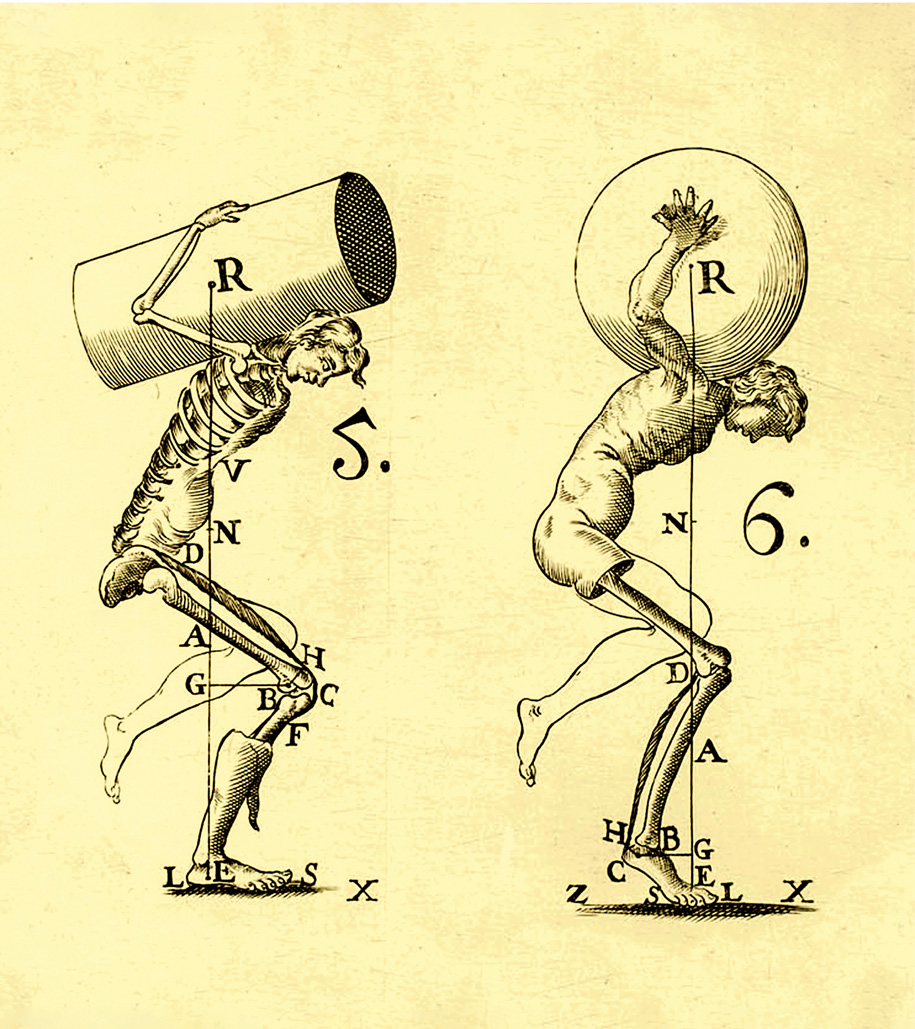
\includegraphics[width=1.0\linewidth]{chap6/6_0}
	% 加星号(*)表示不加编号
	\caption*{ \label{fig:6_0}}
\end{figure}


我读研究生的时候,我的一位导师是尤金$\cdot$布莱克,他是斯坦福医院骨科主任,也是脑瘫骨科治疗书籍的作者。
脑瘫是儿童最常见的残疾原因之一,会影响行走和保持平衡的能力。
脑瘫患者通常会形成一些独特的步态,例如蹲伏步态,这种步态效率低下且费力。


很多情况下,手术延长腿筋可以改善蹲伏步态。
但并非总是如此!我问布莱克医生,他是如何决定是否延长某个病人的腿筋的。
他告诉我,当肌肉“太紧”时,他会进行延长。
他通过观察孩子躺在他的检查床上时,肌肉能被拉伸到什么程度来评估肌肉的紧绷程度。
我走访了不同的医院,发现他们实施手术的标准并不一致。
我想,一定有更好的方法来确定哪些孩子会受益,哪些孩子不会。
问题仅仅是腿筋太短,还是还有其他问题无法通过延长肌肉来解决?


我们在第~\ref{chap:chap4}~章和第~\ref{chap:chap5}~章开始开发的计算机模型非常适合回答这些问题。
在对人体进行不可逆的手术之前,或许我们可以在计算模型上模拟手术。
但我们首先需要在这些模型中添加一些内容:肌肉与骨骼相互作用以产生全身运动的方式。


我们首先要说明的是,肌肉通过向骨骼施加力量来产生运动。
然而,这里有一个微妙之处。
例如,如果你的二头肌恰好附着在肘关节上,你就永远无法移动前臂。
相反,肌肉附着在距离解剖关节一定距离的骨骼上,这样它们就有足够的杠杆作用来移动四肢(如果不是整个世界的话)。
这种杠杆作用称为肌肉的机械优势或力臂。
通过增加肌肉在骨骼上的附着点与关节旋转轴之间的距离,可以增加力臂。
其效果类似于将门把手放置在远离铰链的位置以便于打开门。
肌肉的机械优势由骨骼几何形状、身体姿势和肌肉作用线的路径决定。
我们将这些特征统称为肌肉骨骼几何形状。


正如我们将在本章中看到的,肌肉的机械优势与其在体内的功能密切相关。
因此,不同学科的科学家和临床医生都在研究肌肉骨骼几何学。
古生物学家研究已灭绝动物骨骼化石的形状,以确定肌肉的附着位置,并推断这些动物可能的运动方式。
生物力学家研究世界级运动员的肌肉骨骼几何学,以确定哪些特征使得他们能够取得优异的成绩。
外科医生可以应用肌肉骨骼模型来改善脑瘫患者的生活。


我们将从一个简单的例子开始,但它能让我们更好地理解这些模型的工作原理。
问题是:站立不动需要多大的努力?
哪个更难:将重心放在前脚掌上站立不动,还是将重心集中在双脚中部站立不动?


\section{肌肉机械优势}

为了回答这些问题,我们考虑进行二维静态分析,以了解单块踝关节跖屈肌在安静站立时维持身体直立所需的力量。
我们将身体建模为一个倒立摆,假设身体的整个重量由一条腿支撑,并比较两种情况。
在第一种情况下,人体站立时,其重量均匀分布在脚上,压力中心位于脚跟和脚趾之间的中间位置(图~\ref{fig:6_1},左)。
在第二种情况下,人体向前倾斜,压力中心移向脚趾。


\begin{figure}[!htb]
	\centering
	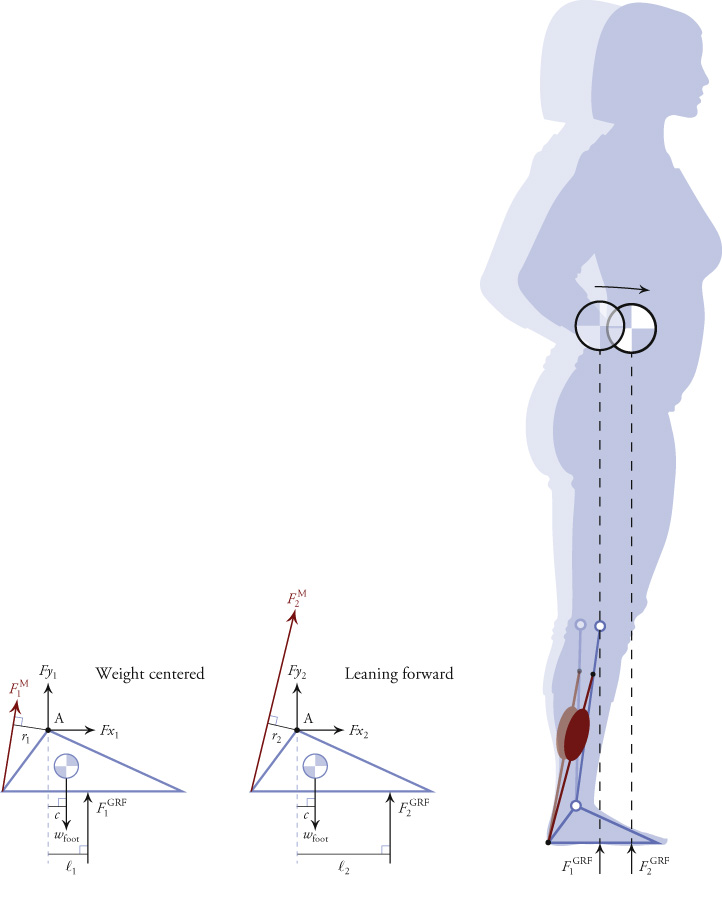
\includegraphics[width=0.9\linewidth]{chap6/6_1}
	\caption{自由体图(左)和模型(右)用于估计人处于直立姿势($F_1^M$)和前倾姿势($F_2^M$)时的跖屈肌力量。 \label{fig:6_1}}
\end{figure}


我们首先绘制每个场景下足部的自由体受力图,并将其与身体其他部位分离,以此开始分析。
我们将足部表示为一个三角形,并假设踝关节位于三角形的上顶点A。
根据阿基米德杠杆定律,我们能够直立而不向前或向后倾倒,这意味着踝关节的力矩总和为零:
%
\begin{equation}
	\sum M_A = F_i ^{\text{GRF}} l_i 
				- w_\text{foot} c
				- F_i ^M r_i
				= 0
	\label{eq:6_1}
\end{equation}
%
索引 $i$ 代表两种情况:1 和 2,即人站立时重心集中在脚上,身体前倾。
重新排列此方程,我们可以计算出肌肉必须产生的力量:
%
\begin{equation}
	F_i ^M = 
		\frac{
			F_i ^{\text{GRF}} l_i
			- w_\text{foot} c
		}{
			r_i
		}
	\label{eq:6_2}
\end{equation}


该方程表明,肌肉中的作用力 ($F_i^M$) 受地面反作用力 ($F_i ^{\text{GRF}}$) 和足部重量 ($w_\text{foot}$) 的大小以及系统几何形状的影响:压力中心的位置 ($l_i$)、足部质心的位置 ($c$),以及值得注意的是从踝关节中心到肌肉力矢量的垂直距离 ($r_i$)。
距离 $r_i$ 定义了肌肉力矩臂。
力矩臂较小的肌肉必须施加更大的力才能产生与力矩臂较大的肌肉相同的关节力矩。
我们说力矩臂较大的肌肉具有更大的机械优势。


表~\ref{tab:6_1}~显示了每种情景下每个变量的实际量。
在第一种情景下,肌肉中的力量大致等于地面反作用力的大小(由于人处于静态平衡状态,因此等于体重)。
在第二种情景下,只需将压力中心向前移动 3 厘米,肌肉力量就会加倍。


\begin{table}[htbp]
	\caption{2 种情况下站立时肌肉力量的计算} \label{tab:6_1} \centering
	\begin{tabular}{ccccccc} % l水平左居中,c水平居中
		\toprule
		场景 & $F_i^{\text{GRF}}$ & $w_\text{foot}$ & $l_i$ & $c$ & $r_i$ & $F_i^M$ \\
		\midrule
		重心($i=1$) & 600牛 &  7.8牛 & 5厘米 & 1厘米 & 5厘米 & 598牛 \\
		\midrule
		向前倾($i=2$) & 600牛 &  7.8牛 & 8厘米 & 1厘米 & 4厘米 & 1198牛 \\
		\bottomrule
	\end{tabular}
\end{table}


请注意,我们平衡了踝关节周围的力矩来计算肌肉力(公式~\ref{eq:6_2})。
如果我们平衡水平和垂直方向的力,就可以计算出关节反作用力的两个分量($F_{x_i}$ 和 $F_{y_i}$)。
我们发现,即使在安静站立时,垂直力($F_{y_i}$)也约为体重的 2-3 倍。
由于肌肉的力臂通常较小,因此存在较大的关节内部接触力;
因此,即使在进行看似毫不费力的任务(例如静止站立或慢行)时,也可能需要较大的肌肉力。


上述示例将力学的基本概念应用于仅涉及一块肌肉的简单二维静态分析。
在下一节中,我们将对力臂进行更正式的工程定义,使其更广泛地应用于三维问题。



\section{肌肉力臂的定义}

在我们对肌肉骨骼几何结构的分析中,我们假设肌肉-肌腱单元可以建模为无摩擦、可伸缩的线,它们附着在骨骼上并缠绕在解剖结构周围。
尽管生物肌肉由数千条纤维组成,每条纤维都有独特的三维路径,但我们通常将肌肉表示为沿着从一个附着点到另一个附着点的路径作用的单一拉力。
该路径决定了肌肉力的作用点以及作用方向。肌肉产生的力矩($ \underline{M} $)可以按如下方式计算(见图~\ref{fig:6_2}):


\begin{figure}[!htb]
	\centering
	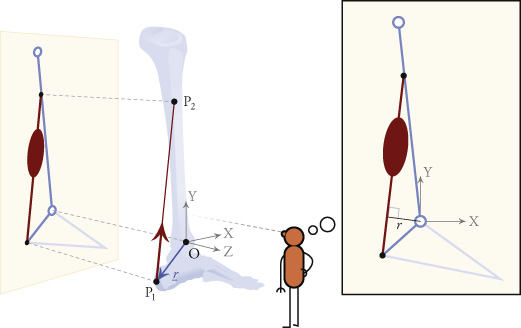
\includegraphics[width=0.9\linewidth]{chap6/6_2}
	\caption{与点 $O$ 处产生力矩有关的力矩臂 $r$ 的定义。 \label{fig:6_2}}
\end{figure}


\begin{equation}
	\underline{M} = \underline{r} \times \underline{F}
	\label{eq:6_3}
\end{equation}
%
其中,“$\times$”表示向量叉积。
点$O$表示关节的旋转中心,向量表示在点$P_1$施加的肌肉力的大小和方向,是从$O$到肌肉作用线上任意一点的向量。


如图~\ref{fig:6_2}~所示,直线肌肉模型的一个吸引人的特性是,$\underline{r}$ 可以从 $O$ 点画到 $P_1$ 点,或者画到 $P_2$ 点,或者画到肌肉作用线上的任何其他点。
在所有情况下,公式~\ref{eq:6_3}~中的叉积结果都相同。
肌肉产生的力矩 ($\underline{M}$) 是一个矢量,但通常更方便地获取标量。
在本例中,我们将公式~\ref{eq:6_3}~投影到 Z 轴上:
%
\begin{equation}
	M_z = ( \underline{r} \times \underline{F} \cdot \hat{z} )
	\label{eq:6_4}
\end{equation}
%
其中“$\cdot$”表示向量点积,$\hat{z}$ 是沿Z轴(与力矩$M_z$相关的旋转轴)的单位向量。
我们通过用肌肉力的大小($r$)对$M_z$进行归一化来定义肌肉的力臂($ \Vert \underline{F} \Vert $):
%
\begin{equation}
	r \triangleq 
		\frac{
			\underline{r} \times \underline{F}
		}{
			\Vert \underline{F} \Vert
		}
		\cdot
		\hat{z}
	\label{eq:6_5}
\end{equation}












